\documentclass[xcolor=table, xcolor=dvipsnames]{beamer}
\usepackage[T1]{fontenc}
\usepackage{amsmath}
\usepackage{amssymb}
\usepackage{mathrsfs}
\usepackage{mathtools}
\usepackage[utf8]{inputenc}
\usepackage{anysize}
\usepackage{graphicx}
\usepackage{wasysym}
\usepackage{xcolor}
\usepackage{hyperref}


\usetheme[secheder]{Boadilla}
\begin{document}
\setbeamertemplate{navigation symbols}{}

\renewcommand{\inserttotalframenumber}{11} 



\title[CLAS12]{CLAS12 PID and Machine Learning}
    \author[Daniel Lersch]{Daniel Lersch, Michael C. Kunkel} 
      \date{$03.10.2017$} 
  %  \logo{\includegraphics[width=1cm]{}}
    \institute[IKP1 - Juelich]
    
    \begin{frame}
      \titlepage
      
       \begin{center}
     \includegraphics[width=0.5\textwidth]{tmva_fun.jpg}
   \end{center}
    \end{frame}
    
%Introduction:    
 %+++++++++++++++++++++++++++++++++++++++++++++++++++++++++++++++++++++++++++++++++++++++++
 \begin{frame}
   \frametitle{\hyperlink{con}{Introduction}}
   \label{intro}
   \footnotesize
   
   \begin{columns}
     \begin{column}{6cm}
       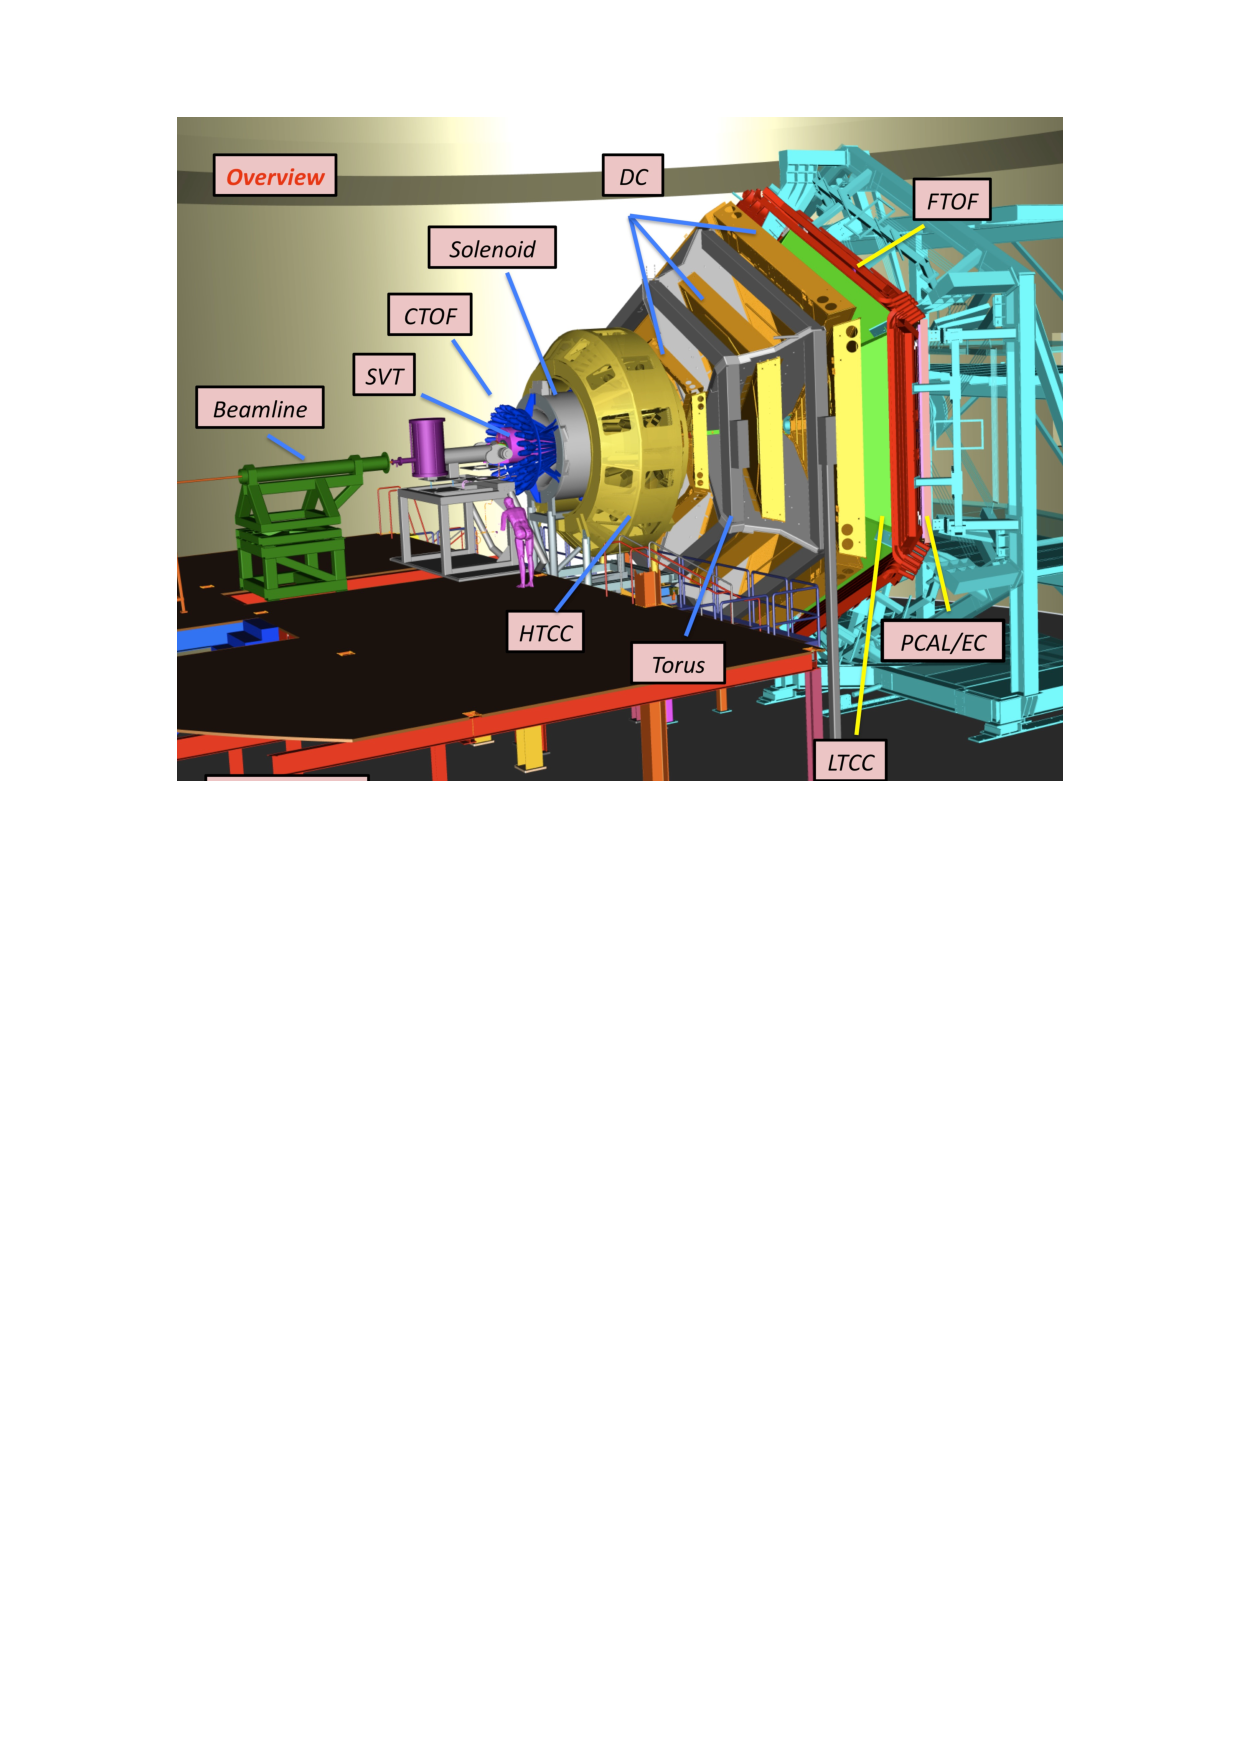
\includegraphics[width=1.05\textwidth]{clas12det.pdf}
     \end{column}
    
     \begin{column}{6cm}
       \begin{itemize}
         \item {\bf Wanted:} Particle masses \\ $m_{e^{\pm}}$, $m_{\pi^{\pm}}$, $m_{p}$, $m_{K^{\pm}}$, ...
         \item {\bf Given:} Information from CLAS12 sub detector systems
         \item {\bf Approach:}  Combine detector information and feed them into a machine learning algorithm \\ $\Rightarrow$ Get particle type
         \item  All results shown here are based on:
         \begin{itemize}
           \footnotesize
           \item Simulated single particle tracks
           \item {\color{blue}{\href{https://gemc.jlab.org/gemc/html/documentation/runningJLab.html} {GEMC 4a.2.1}}}
           \item {\color{blue}{\href{https://github.com/JeffersonLab/clas12-offline-software} {COATJAVA 4a.8.1}}}
           \item {\color{blue}{\href{https://spark.apache.org/} {Apache-Spark 2.20 framework}}} 
         \end{itemize}
       \end{itemize}
      \end{column}
    \end{columns}
    
    \begin{itemize}
      \item[] {\bf $\Rightarrow$ Todays focus:  Separation of $e^{-}$ / $\pi^{-}$}
      \begin{itemize}
        \scriptsize
        \item[i)] Which variables (or combination of variables) to chose for PID?
        \item[ii)]  Which machine learning algorithm / classifier is ''the best``?
        \item[iii)] Quality of results $\Leftrightarrow$ systematic checks?
      \end{itemize}
    \end{itemize}
 \end{frame}
  %+++++++++++++++++++++++++++++++++++++++++++++++++++++++++++++++++++++++++++++++++++++++++    
 
 
 %The Data Set:
 %+++++++++++++++++++++++++++++++++++++++++++++++++++++++++++++++++++++++++++++++++++++++++
 \begin{frame}
  \frametitle{\hyperlink{con}{The $e^{-}\pi^{-}$ Data Set}}
  \label{dataSet}
  \footnotesize
  
    \includegraphics[width=1.02\textwidth,height=0.53\textwidth]{pidCorrPlotsAll.png}
 
  \begin{itemize}
   \item Possible PID-variables: \\ {\bf p}, {\bf nphe(LTCC)}, {\bf nphe(HTCC)}, {\bf $\Delta E(pcal)$}, {\bf $\Delta E(ec:in)$}, {\bf $\Delta E(ec:out)$}, {\bf $\Delta E(cal)$}, {\bf t}
   \item Ratio: $N(\pi^{-}) / N(e^{-}) = 10$
   \item Request particles to have: $p > 0$ and at least one other sub detector fired
  \end{itemize}
 \end{frame}
 %+++++++++++++++++++++++++++++++++++++++++++++++++++++++++++++++++++++++++++++++++++++++++
 
 
 
 %Classifier Scheme:
 %+++++++++++++++++++++++++++++++++++++++++++++++++++++++++++++++++++++++++++++++++++++++++
\begin{frame}
  \frametitle{\hyperlink{con}{Solving multivariate Classification Problems}}
  \label{classi}
  \footnotesize
  
  \begin{itemize} 
    \item Several classifier algorithms available \\ (neural networks, boosted decision trees, support vector machines,...)
    \item Classifier internal parameters (weights, thresholds,...) are determined via training
  \end{itemize}
  
  \includegraphics[width=1.0\textwidth,height=0.57\textwidth]{classifier_scheme_new.pdf}
\end{frame}
%+++++++++++++++++++++++++++++++++++++++++++++++++++++++++++++++++++++++++++++++++++++++++


%Roc-Curve:
%+++++++++++++++++++++++++++++++++++++++++++++++++++++++++++++++++++++++++++++++++++++++++
\begin{frame}
 \frametitle{\hyperlink{con}{Evaluation of a trained Classifier: The ROC-Curve}}
 \label{rocCurve}
 \scriptsize
 
 \alt<1>{
  \begin{figure}
    \includegraphics[width=1.0\textwidth]{rocCurveMLP_HL85V123456N6000R1.png}
  \end{figure}
 }{}
 
  \alt<2>{
  \begin{figure}
    \includegraphics[width=1.0\textwidth]{rocCurveMLP_HL85V123456N6000R1_EX1.png}
  \end{figure}
 }{}
 
  \alt<3>{
  \begin{figure}
    \includegraphics[width=1.0\textwidth]{rocCurveMLP_HL85V123456N6000R1_EX2.png}
  \end{figure}
 }{}
 
  \alt<4>{
  \begin{figure}
    \includegraphics[width=1.0\textwidth]{rocCurveMLP_HL85V123456N6000R1_EX3.png}
  \end{figure}
 }{}

 \begin{columns}
 \begin{column}{7cm}
 \begin{itemize}
  \item \underline{Receiver-Operating-Characteristics:}
  \begin{itemize}
    \scriptsize
    \item {\bf Efficiency}: $\epsilon_{S} = \frac{N^{acc}_{S}}{N^{all}_{S}}$, $\epsilon_{B} = \frac{N^{rej}_{B}}{N^{all}_{B}}$
    \item {\bf Purity}: $P_S = \frac{N^{acc}_{S}}{N^{acc}_{S} + N^{acc}_{B}}$, $P_B = \frac{N^{acc}_{B}}{N^{acc}_{S} + N^{acc}_{B}}$
    \item {\bf False Positive Rate}: $FPR =  \frac{N^{acc}_{B}}{N^{all}_{B}}$
    \item {\bf False Negative Rate}: $FPR =  \frac{N^{rej}_{S}}{N^{all}_{S}}$
  \end{itemize}
 \end{itemize}
 \end{column}
 
 \begin{column}{5cm}
  \includegraphics[width=1.05\textwidth,height=0.65\textwidth]{probMLP_HL85V123456N6000R1.png}
 \end{column}
 \end{columns}
\end{frame}
%+++++++++++++++++++++++++++++++++++++++++++++++++++++++++++++++++++++++++++++++++++++++++

%Roc-Metric:
%+++++++++++++++++++++++++++++++++++++++++++++++++++++++++++++++++++++++++++++++++++++++++
\begin{frame}
  \frametitle{\hyperlink{con}{Choosing the Classification Parameters: ROC-Metrics}}
  \label{rocMetric}
    
     \scriptsize
  \begin{itemize}
   \item Use ROC-curve to:
   \begin{itemize}
     \scriptsize
     \item[i)] Select probability cut
     \item[ii)] Choose classifier
   \end{itemize}
    \item Apply metric:
    \begin{itemize}
      \scriptsize
      \item Distance: $d \equiv \sqrt{(1-\epsilon_S)^2 + (0-FPR)^2} \in [0,\infty)$ {\color{gray}{(left plot)}}
      \item {\color{blue}{\href{https://en.wikipedia.org/wiki/F1_score}{F1 score:}}} $f_1 \equiv 2\frac{\epsilon_S\times P_S}{\epsilon_S + P_S} \in [0,1]$ {\color{gray}{(centre plot)}}
      \item {\color{blue}{\href{https://en.wikipedia.org/wiki/Matthews_correlation_coefficient}{Mathews Correlation Coefficient:}}} $MCC \equiv \frac{\epsilon_S\times \epsilon_B - FPR\times FNR}{\sqrt{ \frac{\epsilon_S}{P_S} \times \frac{\epsilon_B}{P_B} } } \in [-1,1]$ {\color{gray}{(right plot)}}
    \end{itemize}
   \end{itemize}  
    
    \begin{figure}
    \includegraphics[width=1.03\textwidth]{rocMetricMLP_HL85V123456N6000R1.png}
    \end{figure}
  \end{frame}
%+++++++++++++++++++++++++++++++++++++++++++++++++++++++++++++++++++++++++++++++++++++++++

%Roc-Metric:
%+++++++++++++++++++++++++++++++++++++++++++++++++++++++++++++++++++++++++++++++++++++++++
\begin{frame}
  \frametitle{\hyperlink{con}{Choosing the Classification Parameters: Result}}
  \label{rocRes}
  \footnotesize
  
  \begin{columns}
    \begin{column}{5cm}
     \includegraphics[width=0.99\textwidth]{logEntry1.jpg}
    \end{column}
 
  
   \begin{column}{7cm}
        \begin{itemize}
    \item Use MCC to choose a classifier, PID Variables and probability threshold:
    \begin{itemize}
      \scriptsize
      \item Boosted Decision Tree with 100 Trees and probability threshold: $0.48$
      \item Neural Network with architecture $\{8 : 5\}$ and probability threshold: $0.57$
      \item Both classifier trained with:
      \begin{itemize}
        \scriptsize
        \item  $p$
        \item nphe(LTCC)
        \item nphe(HTCC)
        \item $\Delta E(pcal)$
        \item $\Delta E(ec:in)$
        \item $\Delta E(ec:out)$
        \item $N(\pi^{-}) / N(e^{-}) = 1$
      \end{itemize}   
   \end{itemize}
   \item Room for improvement: Automated Parameter Scan as a function of MCC \\ (Or any other metric)
     \end{itemize}
   \end{column}
 \end{columns}
\end{frame}
%+++++++++++++++++++++++++++++++++++++++++++++++++++++++++++++++++++++++++++++++++++++++++



%Results after PID:
%+++++++++++++++++++++++++++++++++++++++++++++++++++++++++++++++++++++++++++++++++++++++++
\begin{frame}
  \frametitle{\hyperlink{con}{Application of the Classifier on the $e^{-}\pi^{-}$ Data Set}}
  \label{app}
   \footnotesize
   
   \alt<1>{
   \begin{figure}
    \includegraphics[width=1.03\textwidth]{pidCALT_raw.png}
   \end{figure}
   
     \begin{table}
      \begin{tabular}{c||c||c||c||c}
     {\bf Classifier} & {\bf Efficiency $\epsilon_S$  $[\%]$} & {\bf Purity $P_S$ $[\%]$} & {\bf FPR $[\%]$} & {\bf $[N(\pi^-)/N(e^-)]_{rec}$} \\
      \hline
      \hline
     {\color{white}{  Decision Tree}} & $-$ & $-$ & $-$ & $-$ \\
      \hline
       {\color{white}{ Neural Network}} & $-$ & $-$ & $-$ & $-$  \\
      \end{tabular}
    \end{table}
   }{}
   
    \alt<2>{
   \begin{figure}
    \includegraphics[width=1.03\textwidth]{pidCALTMLP_HL85V123456N6000R1.png}
   \end{figure}
   
     \begin{table}
      \begin{tabular}{c||c||c||c||c}
     {\bf Classifier} & {\bf Efficiency $\epsilon_S$  $[\%]$} & {\bf Purity $P_S$ $[\%]$} & {\bf FPR $[\%]$}  & {\bf $[N(\pi^-)/N(e^-)]_{rec}$} \\
      \hline
      \hline
      Decision Tree & $96$ & $58$ & $7$ &  $6$ \\
      \hline
      Neural Network & $94$ & $61$ & $6$ & $6$ \\
      \end{tabular}
    \end{table}
   }{}       
     
\end{frame}
%+++++++++++++++++++++++++++++++++++++++++++++++++++++++++++++++++++++++++++++++++++++++++

%Magnetic Field:
%+++++++++++++++++++++++++++++++++++++++++++++++++++++++++++++++++++++++++++++++++++++++++
\begin{frame}
  \frametitle{\hyperlink{con}{Changing the Magnetic Field}}
  \label{mField}
  \scriptsize
  
  \begin{itemize}
    \item Checked influence of different magnetic field settings on classifier performance
    \item Kept ratio: $N(\pi^-) / N(e^-) = 10$
    \item Three numbers in each cell of the table are:
    \\$\epsilon_S [\%]$  / $P_S [\%]$ / $FPR [\%]$
  \end{itemize}
  
  \begin{table}
     \scriptsize
    \begin{tabular}{c||c|c|c}
 
      {\bf Applied Field $\Rightarrow$}  & $Tor. =-1$  &  $Tor. =-0.75$ &  $Tor. =-0.75$  \\
      {\bf Trained Field $\Downarrow$} & $Sol. =1$ &   $Sol. =0.6$ &  $Sol. =0.8$ \\
      \hline
      \hline
       $Tor. =-1$ &  $94$ / $61$ / $6$  &  $95$ / $62$ / $6$  & $95$ / $61$ / $6$ \\
       $Sol. =1$ &    &    & \\
       \hline 
        $Tor. =-0.75$ &  $94$ / $53$ / $8$  &  $95$ / $57$ / $8$  & $95$ / $55$ / $8$ \\
         $Sol. =0.6$ &   &   & \\
        \hline
         $Tor. =-0.75$  &  $95$ / $56$ / $6$  &  $95$ / $59$ / $6$  & $95$ / $57$ / $7$ \\
          $Sol. =0.8$ &   &   & \\
    \end{tabular}
  \end{table}
  
\includegraphics[width=0.4\textwidth,origin=l]{pidMLP_HL85V123456N6000R1_trueMomentum.png}
\includegraphics[width=0.39\textwidth,origin=r]{pidMLP_T-1S1_trueT-075S08Momentum.png}

  
\end{frame}
%+++++++++++++++++++++++++++++++++++++++++++++++++++++++++++++++++++++++++++++++++++++++++

%Smearing:
%+++++++++++++++++++++++++++++++++++++++++++++++++++++++++++++++++++++++++++++++++++++++++
\begin{frame}
  \frametitle{\hyperlink{con}{Resolution Effects for $N(\pi^{-}) / N(e^{-}) = 1$}}
  \label{smear}
  \scriptsize
  
  \alt<1>{
   \begin{figure}
     \includegraphics[width=1.0\textwidth]{rocNoSmear.png}
   \end{figure}
   
    \begin{itemize}
    \item {\bf Basic question:} What happens if resolution in measured data is different from the resolution the classifier has been trained on?
    \item {\bf Simple Test:} Apply trained classifier on a data set with different resolution than the training set
    \item Smeared all PID variables by a Gaussian distribution: $x \mapsto x + \text{Gauss(0, $\delta \cdot x$)}$
    \item Shown above: ROC-curves for $\delta = 0.0$
  \end{itemize}
  }{}
  
   \alt<2>{
   \begin{figure}
     \includegraphics[width=1.0\textwidth]{rocSmear005.png}
   \end{figure}
   
    \begin{itemize}
    \item {\bf Basic question:} What happens if resolution in measured data is different from the resolution the classifier has been trained on?
    \item {\bf Simple Test:} Apply trained classifier on a data set with different resolution than the training set
    \item Smeared all PID variables by a Gaussian distribution: $x \mapsto x + \text{Gauss(0, $\delta \cdot x$)}$
    \item Shown above: ROC-curves for $\delta = 5\%$
  \end{itemize}
  }{}
  
   \alt<3>{
   \begin{figure}
     \includegraphics[width=1.0\textwidth]{rocSmear015.png}
   \end{figure}
   
    \begin{itemize}
    \item {\bf Basic question:} What happens if resolution in measured data is different from the resolution the classifier has been trained on?
    \item {\bf Simple Test:} Apply trained classifier on a data set with different resolution than the training set
    \item Smeared all PID variables by a Gaussian distribution: $x \mapsto x + \text{Gauss(0, $\delta  \cdot x$)}$
    \item Shown above: ROC-curves for $\delta = 15\%$
  \end{itemize}
  }{}
  
     \alt<4>{
   \begin{figure}
     \includegraphics[width=1.0\textwidth]{rocSmear025.png}
   \end{figure}
   
    \begin{itemize}
    \item {\bf Basic question:} What happens if resolution in measured data is different from the resolution the classifier has been trained on?
    \item {\bf Simple Test:} Apply trained classifier on a data set with different resolution than the training set
    \item Smeared all PID variables by a Gaussian distribution: $x \mapsto x + \text{Gauss(0, $\delta \cdot x$)}$
    \item Shown above: ROC-curves for $\delta = 25\%$
  \end{itemize}
  }{} 
  
    \alt<5>{
   \begin{figure}
     \includegraphics[width=1.0\textwidth]{rocSmear035.png}
   \end{figure}
   
    \begin{itemize}
    \item {\bf Basic question:} What happens if resolution in measured data is different from the resolution the classifier has been trained on?
    \item {\bf Simple Test:} Apply trained classifier on a data set with different resolution than the training set
    \item Smeared all PID variables by a Gaussian distribution: $x \mapsto x + \text{Gauss(0, $\delta  \cdot x$)}$
    \item Shown above: ROC-curves for $\delta = 35\%$
  \end{itemize}
  }{} 

\end{frame}
%+++++++++++++++++++++++++++++++++++++++++++++++++++++++++++++++++++++++++++++++++++++++++



%Summary and Outlook:
%+++++++++++++++++++++++++++++++++++++++++++++++++++++++++++++++++++++++++++++++++++++++++
\begin{frame}
 \frametitle{\hyperlink{con}{Summary and Outlook}}
 \label{fin}
 \footnotesize
 
 \begin{itemize}
 \item[\CheckedBox] Set up  and use Machine Learning for PID
  \item[\CheckedBox] Performed identification of $e^{-}$ in a $\pi^{-}$-dominated data set
  \begin{itemize}
  \scriptsize
    \item Key variables: $p$, nphe(LTCC), nphe(HTCC), $\Delta E(pcal)$, $\Delta E(ec:in)$, $\Delta E(ec:out)$
    \item Use two classifier $\Rightarrow$ chosen by ROC-metric $\Rightarrow$ Both performed equally: $\epsilon_{e^{-}} \sim 95\%$
    \item Checked influence of magnetic field settings $\Rightarrow$ No significant impact indicated
    \item Studied resolution effects $\Rightarrow$ In this analysis: managable performance for $\delta < 15\%$
  \end{itemize}
  \item[$\Box$] Test methods on KPP-Data
  \item[$\Box$] Perform PID studies for $e^{+}$, $\pi^{+}$, $K^{\pm}$ and $p$ (ongoing)
  \item[$\Box$] Estimation of Variable Importance (ongoing)
  \item[$\Box$] Include further classifier algorithms (e.g. SVM, Likelihood,...) (ongoing)
  \item[$\Box$] Possible X-check of PID-results (e.g. compare $\beta$(PID) with $\beta$(ToF))
 \end{itemize}
 
 \begin{figure}
 \includegraphics[width=0.4\textwidth]{betaVsMom.png}
 \end{figure}
\end{frame}
%+++++++++++++++++++++++++++++++++++++++++++++++++++++++++++++++++++++++++++++++++++++++++


%########################################################################################################
%########################################################################################################
%########################################################################################################

%Content:
%+++++++++++++++++++++++++++++++++++++++++++++++++++++++++++++++++++++++++++++++++++++++++
\begin{frame}
  \frametitle{Content}
  \label{con}
  \footnotesize
  
  \begin{itemize}
    \item[1.] \hyperlink{intro}{Introduction} {\color{blue}{(\ref{intro})}}
    \item[2.] \hyperlink{dataSet}{The $e^{-}\pi^{-}$ Data Set} {\color{blue}{(\ref{dataSet})}}
    \item[3.] \hyperlink{classi}{Solving multivariate Classification Problems}  {\color{blue}{(\ref{classi})}} 
    \item[4.] \hyperlink{rocCurve}{Evaluation of a trained Classifier: The ROC-Curve}  {\color{blue}{(\ref{rocCurve})}} 
    \item[5.] \hyperlink{rocMetric}{Choosing the Classification Parameters: ROC-Metrics}  {\color{blue}{(\ref{rocMetric})}} 
    \item[6.] \hyperlink{rocRes}{Choosing the Classification Parameters: Result}  {\color{blue}{(\ref{rocRes})}} 
    \item[7.] \hyperlink{app}{Application of the Classifier on the $e^{-}\pi^{-}$ Data Set}  {\color{blue}{(\ref{app})}} 
    \item[8.] \hyperlink{mField}{Changing the Magnetic Field} {\color{blue}{(\ref{mField})}} 
    \item[9.] \hyperlink{smear}{Resolution Effects for $N(\pi^{-}) / N(e^{-}) = 1$}  {\color{blue}{(\ref{smear})}} 
    \item[10.] \hyperlink{fin}{Summary and Outlook} {\color{blue}{(\ref{fin})}} 
  \end{itemize}
\end{frame}
%+++++++++++++++++++++++++++++++++++++++++++++++++++++++++++++++++++++++++++++++++++++++++

%Backup
%+++++++++++++++++++++++++++++++++++++++++++++++++++++++++++++++++++++++++++++++++++++++++
\begin{frame}
 \frametitle{Backup Stuff}
 \label{bup}
 \footnotesize
 
 \begin{itemize}
   \item[1.] \hyperlink{bdataSet}{The $e^{-}\pi^{-}$ Data Set} {\color{blue}{(\ref{bdataSet})}}
   \item[2.] \hyperlink{1dDists}{1D Distributions before and after PID} {\color{blue}{(\ref{1dDists})}}
   \item[3.] \hyperlink{1dDistsTrue}{Compare True and ID Distributions} {\color{blue}{(\ref{1dDistsTrue})}}
   \item[4.] \hyperlink{1dDistsTrueTrue}{Compare True and ID Distributions for true Electrons} {\color{blue}{(\ref{1dDistsTrueTrue})}}
   \item[5.] \hyperlink{compPid}{Comparison of PID-Plots} {\color{blue}{(\ref{compPid})}}
   \item[6.] \hyperlink{ratio}{Useful Relations} {\color{blue}{(\ref{ratio})}} 
   \item[7.] \hyperlink{readConf}{Generating single Track Training Data}  {\color{blue}{(\ref{readConf})}} 
   \item[8.] \hyperlink{trainConf}{Training and Choice of the Classifier} {\color{blue}{(\ref{trainConf})}} 
   \item[9.] \hyperlink{train}{Training a Classifier}  {\color{blue}{(\ref{train})}} 
   \item[10.] \hyperlink{bmField}{Backup: Changing the Magnetic Field} {\color{blue}{(\ref{bmField})}} 
 \end{itemize}
 
\end{frame}
%+++++++++++++++++++++++++++++++++++++++++++++++++++++++++++++++++++++++++++++++++++++++++

%2D-Plots:
%+++++++++++++++++++++++++++++++++++++++++++++++++++++++++++++++++++++++++++++++++++++++++
\begin{frame}
  \frametitle{\hyperlink{bup}{Backup: The $e^{-}\pi^{-}$ Data Set}}
  \label{bdataSet}
   \alt<1>{
    \framesubtitle{All Particles}
     \begin{figure}
        \includegraphics[width=1.03\textwidth,height=0.5\textwidth]{pidCorrPlotsAll.png}
     \end{figure}
  }{}
  \alt<2>{
  \framesubtitle{Electrons}
     \begin{figure}
        \includegraphics[width=1.03\textwidth,height=0.5\textwidth]{pidCorrPlotsSig.png}
     \end{figure}
  }{}
   \alt<3>{
   \framesubtitle{Negative Pions}
     \begin{figure}
        \includegraphics[width=1.03\textwidth,height=0.5\textwidth]{pidCorrPlotsBkg.png}
     \end{figure}
  }{}
\end{frame}
%+++++++++++++++++++++++++++++++++++++++++++++++++++++++++++++++++++++++++++++++++++++++++


%Results:
%+++++++++++++++++++++++++++++++++++++++++++++++++++++++++++++++++++++++++++++++++++++++++
\begin{frame}
  \frametitle{\hyperlink{bup}{Backup: 1D Distributions before and after PID}}
  \label{1dDists}
  \footnotesize
   
   \alt<1>{
   \begin{figure}
     \includegraphics[width=1.02\textwidth,height=0.5\textwidth]{pidMLP_HL85V123456N6000R1_all.png}
   \end{figure}
   
   Apply neural network algorithm on $e^{-}\pi^{-}$ data set:
   \begin{itemize}
      \item $\epsilon_S = 94\%$
      \item $P_S = 62\%$
   \end{itemize}
   }{}
   
    \alt<2>{
   \begin{figure}
     \includegraphics[width=1.02\textwidth,height=0.5\textwidth]{pidGBT_V123456R1_all.png}
   \end{figure}
   
   Apply boosted decision tree algorithm on $e^{-}\pi^{-}$ data set:
   \begin{itemize}
      \item $\epsilon_S = 96\%$
      \item $P_S = 58\%$
   \end{itemize}
   }{}
\end{frame}
%+++++++++++++++++++++++++++++++++++++++++++++++++++++++++++++++++++++++++++++++++++++++++

%True vs. Rec:
%+++++++++++++++++++++++++++++++++++++++++++++++++++++++++++++++++++++++++++++++++++++++++
\begin{frame}
  \frametitle{\hyperlink{bup}{Backup: Compare True and ID Distributions}}
  \label{1dDistsTrue}
   \footnotesize
   
  \alt<1>{
    \begin{figure}
      \includegraphics[width=1.02\textwidth,height=0.5\textwidth]{pidMLP_HL85V123456N6000R1.png}
    \end{figure}
    
    Apply neural network algorithm on $e^{-}\pi^{-}$ data set:
   \begin{itemize}
      \item $\epsilon_S = 94\%$
      \item $P_S = 62\%$
   \end{itemize}    
  }{}
  
    \alt<2>{
   \begin{figure}
     \includegraphics[width=1.02\textwidth,height=0.5\textwidth]{pidGBT_V123456R1.png}
   \end{figure}
   
   Apply boosted decision tree algorithm on $e^{-}\pi^{-}$ data set:
   \begin{itemize}
      \item $\epsilon_S = 96\%$
      \item $P_S = 58\%$
   \end{itemize}
   }{}  
\end{frame}
%+++++++++++++++++++++++++++++++++++++++++++++++++++++++++++++++++++++++++++++++++++++++++

%True vs. Rec for true Electrons:
%+++++++++++++++++++++++++++++++++++++++++++++++++++++++++++++++++++++++++++++++++++++++++
\begin{frame}
  \frametitle{\hyperlink{bup}{Backup: Compare True and ID Distributions for true Electrons}}
  \label{1dDistsTrueTrue}
   \footnotesize
  
  \alt<1>{
    \begin{figure}
      \includegraphics[width=1.0\textwidth,height=0.45\textwidth]{pidMLP_HL85V123456N6000R1_true.png}
    \end{figure}
    
    Apply neural network algorithm on $e^{-}\pi^{-}$ data set:
   \begin{itemize}
      \item $\epsilon_S = 94\%$
      \item $P_S = 62\%$
   \end{itemize}    
  }{}
  
    \alt<2>{
   \begin{figure}
     \includegraphics[width=1.0\textwidth,height=0.45\textwidth]{pidGBT_V123456R1_true.png}
   \end{figure}
   
   Apply boosted decision tree algorithm on $e^{-}\pi^{-}$ data set:
   \begin{itemize}
      \item $\epsilon_S = 96\%$
      \item $P_S = 58\%$
   \end{itemize}
   }{}  
\end{frame}
%+++++++++++++++++++++++++++++++++++++++++++++++++++++++++++++++++++++++++++++++++++++++++

%GBT:pidCALT
%+++++++++++++++++++++++++++++++++++++++++++++++++++++++++++++++++++++++++++++++++++++++++
\begin{frame}
  \frametitle{\hyperlink{bup}{Backup: Comparison of PID-Plots}}
  \label{compPid}
  \footnotesize
  
  \begin{figure}
    \includegraphics[width=0.85\textwidth]{pidCALTMLP_HL85V123456N6000R1.png}\\
   \includegraphics[width=0.85\textwidth]{pidCALT_GBTV123456R1.png}
  \end{figure}
  Top: MLP / Bottom: GBT
  
\end{frame}
%+++++++++++++++++++++++++++++++++++++++++++++++++++++++++++++++++++++++++++++++++++++++++



%Dependencies:
%+++++++++++++++++++++++++++++++++++++++++++++++++++++++++++++++++++++++++++++++++++++++++
\begin{frame}
  \frametitle{\hyperlink{bup}{Backup: Useful Relations}}
  \label{ratio}
  \footnotesize
  
  
  \begin{itemize}
    \item $\epsilon_S$ and FPR are features of the classifier and (ideally) independent of the ratio between the species
    \item $\Big( \frac{N^{all}_{B}}{N^{all}_{S}} \Big)_{rec} =  \Big[ \frac{P_S}{\epsilon_S} \times \frac{\epsilon_B}{P_B}\Big] \times \Big( \frac{N^{all}_{B}}{N^{all}_{S}} \Big)_{true}$
    \item $P_S = \epsilon_S \times \Big [ \epsilon_S + FPR \times \Big( \frac{N^{all}_{B}}{N^{all}_{S}} \Big)_{true} \Big]^{-1}$
  \end{itemize}
  
  \includegraphics[width=0.65\textwidth]{rocEXR1.png} \\
  \includegraphics[width=0.65\textwidth]{rocEXR01.png}
  
\end{frame}
%+++++++++++++++++++++++++++++++++++++++++++++++++++++++++++++++++++++++++++++++++++++++++

%Generating Training Data:
%+++++++++++++++++++++++++++++++++++++++++++++++++++++++++++++++++++++++++++++++++++++++++
\begin{frame}
  \frametitle{\hyperlink{bup}{Backup: Generating single Track Training Data}}
  \label{readConf}
 \scriptsize
  
  \begin{figure}
    \includegraphics[width=0.99\textwidth]{testConf2.png}
  \end{figure}
  
  \begin{itemize}
    \item Java-based Module:
    \begin{itemize}
      \scriptsize
      \item Generate training data from reconstructed CLAS12 data
      \item Test a classifier on reconstructed CLAS12 data
      \item Can be run by/with multiple users/configurations
    \end{itemize}
    \item Module parameters are specified in a txt-file (see top figure)
    \item Txt-file generation and submission to farm are run by a single script
  \end{itemize}
\end{frame}
%+++++++++++++++++++++++++++++++++++++++++++++++++++++++++++++++++++++++++++++++++++++++++

%Training Module:
%+++++++++++++++++++++++++++++++++++++++++++++++++++++++++++++++++++++++++++++++++++++++++
\begin{frame}
  \frametitle{\hyperlink{bup}{Backup: Training and Choice of the Classifier}}
  \label{trainConf}
  \scriptsize
  
   \begin{figure}
    \includegraphics[width=0.55\textwidth]{trainConf2.png}
  \end{figure}
  
  \begin{itemize}
    \item Java-based Module:
    \begin{itemize}
      \scriptsize
      \item Specify the variables used for training
      \item Select the classifier that shall be trained
      \item Define how the classifier shall be trained 
      \item Can be run by/with multiple users/configurations
    \end{itemize}
    \item Module parameters are specified in a txt-file (see top figure)
     \item Txt-file generation and submission to farm are run by a single script
  \end{itemize}
\end{frame}
%+++++++++++++++++++++++++++++++++++++++++++++++++++++++++++++++++++++++++++++++++++++++++

%Training:
%+++++++++++++++++++++++++++++++++++++++++++++++++++++++++++++++++++++++++++++++++++++++++
\begin{frame}
 \frametitle{\hyperlink{bup}{Backup: Training a Classifier}}
 \label{train}
 \footnotesize
 
 \begin{figure}
   \includegraphics[width=0.9\textwidth]{training_example.pdf}
 \end{figure}
\end{frame}
%+++++++++++++++++++++++++++++++++++++++++++++++++++++++++++++++++++++++++++++++++++++++++

%Magnetic field:
%+++++++++++++++++++++++++++++++++++++++++++++++++++++++++++++++++++++++++++++++++++++++++
\begin{frame}
  \frametitle{\hyperlink{bup}{Backup: Changing the Magnetic Field}}
  \label{bmField}
  \footnotesize
  
  \begin{figure}
    \includegraphics[width=0.7\textwidth]{pidCALTMLP_T-075S08.png}\\
     \includegraphics[width=0.7\textwidth]{pidCALTMLP_T-075S08_appT-1S1.png}
  \end{figure}
  
  \begin{itemize}
    \item Top: Classifier trained on: Tor. = $-0.75$ and Sol. = $0.8$ and applied on: Tor. = $-0.75$ and Sol. = $0.8$
    \item Bottom: Classifier trained on: Tor. = $-0.75$ and Sol. = $0.8$ and applied on: Tor. = $-1$ and Sol. = $1$
  \end{itemize}
  
\end{frame}
%+++++++++++++++++++++++++++++++++++++++++++++++++++++++++++++++++++++++++++++++++++++++++


    
  
%%%%%%%%%%%%%%%%%%%%%%%%%%%%%%%%%%%%%%%%%%%%%%%%%%%%%%%%%%%







 \end{document}